%% -*- coding: utf-8 -*-
\documentclass[12pt,pagesize,paper=192mm:108mm]{scrbook} 
%1920x1080 1280x720
\areaset[current]{192mm}{108mm}
\usepackage{calc}
\usepackage[T2A]{fontenc}
\usepackage[utf8]{inputenc}
\usepackage[english,russian]{babel}
\usepackage{microtype}
\usepackage{misccorr}
\usepackage{cmap}
%\usepackage[unicode=true]{hyperref}
\usepackage{graphicx}
\usepackage{amssymb}
\usepackage{amsmath}
%\usepackage{srcltx}
\usepackage{textcomp}
\usepackage{xspace}
%научные символы и смайлики \smiley \frownie
\usepackage{wasysym}
\usepackage{ccicons}
\begin{document}
\begin{titlepage}
  \vspace*{-0.5em}
  \begin{center}    
    \hspace*{3em}
    \begin{minipage}[t]{3em}
      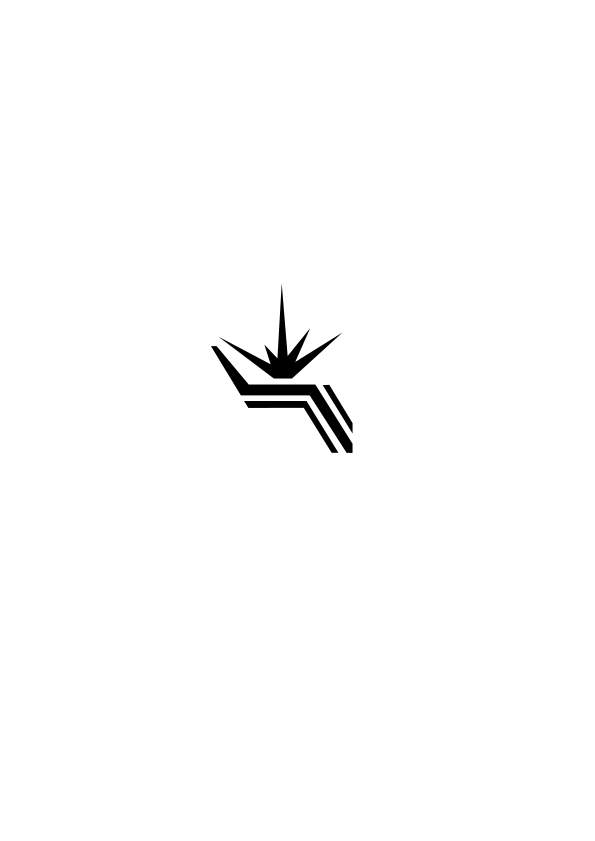
\includegraphics[width=\textwidth]{../BINP-logo}
    \end{minipage}\hfill
    \begin{minipage}{0.23\linewidth}
    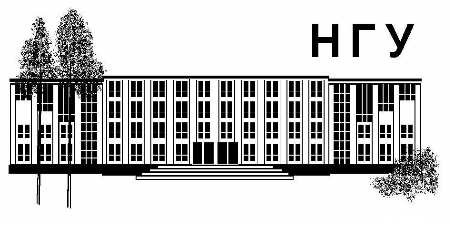
\includegraphics[width=\textwidth]{../NSU-logo}
    \end{minipage}
    \hfill
    \hspace*{6em}

    Кафедра теоретической физики физического факультета НГУ
    \medskip

    \Large
    Профессор Черняк В.\,Л.
    \bigskip

    \huge
    \textbf{Теория электрослабых взаимодействий}
    \bigskip

    \Large
    Лекция № 8
    \vfill

    % \normalsize
    % \begin{minipage}{0.65\linewidth}
    % \end{minipage}
    \vfill

\normalsize    Новосибирск 2013
  \smallskip

  \ccbysa
  \end{center}
\end{titlepage}
\newpage

\vspace*{-1em}
\begin{center}
 \vfill
  \begin{minipage}{0.66\linewidth}
    Полная ширина распада $W$"=бозона. КХД"=поправки к данному
    распаду. Ширина распада $Z$"=бозона. Слабые процессы второго
    порядка.  Рассеяние электрона на кварке. Схема вычисления ширины
    распада мюона на электрон, электронное антинейтрино и мюонное
    нейтрино.  Константа Ферми. Лагранжиан Ферми. Лептонные слабые
    процессы. Распад $\pi$"=мезона на электрон и электронное
    антинейтрино, а также мюон и мюонное антинейтрино. Адронные
    матричные элементы. Константа $f_{\pi}$.  Отношение электронной и
    мюонной ширин. Качественное объяснение пропорциональности этого
    отношения квадратам масс.
  \end{minipage}
  \vfill
  % Новосибирск 2013

  % \normalsize \ccbysa
\end{center}
\end{document}
